\documentclass[a0paper,portrait,20pt]{extarticle}

\usepackage[margin=2cm]{geometry}
\usepackage[T1]{fontenc}
% \usepackage{lmodern}
\usepackage{helvet} % scalable sans font (Nimbus Sans)
\renewcommand{\familydefault}{\sfdefault}
\usepackage{anyfontsize}
\usepackage{graphicx}
\usepackage{amsmath,amssymb}
\usepackage{xcolor}
\usepackage{float}
\usepackage[most]{tcolorbox}
\usepackage[backend=biber,style=authoryear]{biblatex}

\addbibresource{references.bib}

\pagestyle{empty}
\setlength{\parindent}{0pt}
\setlength{\parskip}{0.6em}

\usepackage{multicol}
\columnsep=50pt
% ------------------------------------------------------------
% Colours and title box style
% ------------------------------------------------------------
% 
\definecolor{posterblue}{HTML}{1F4E79}
\definecolor{posterbg}{HTML}{EAF1F8}
 
%Header titlebox
\tcbset{titlebox/.style={enhanced, colframe=posterbg,
    colback=posterbg,
    boxrule=3pt,
    %arc=4pt,
    left=2cm, right=2cm, top=1.5cm, bottom=1.5cm,
    width=\textwidth,
    %halign=center
  }
}

% Footer titlebox
\newtcolorbox{footerbox}{enhanced,
  colframe=posterblue,
  colback=white,
  boxrule=3pt,
  left=20pt, right=20pt, top=12pt, bottom=12pt,
  width=\textwidth
}

% Defining a custom environment called 'nofillbox'
\newtcolorbox{nofillbox}[1]{
  enhanced,
  colback=white,            % Makes the background completely transparent
  colframe=posterblue,     % Border color
  % coltitle=,     % Title text color
  %fonttitle=\bfseries,     % Bold title
  left=20pt, right=20pt, top=12pt, bottom=12pt,
  boxrule=3pt,             % Slim border outline
  title={#1},               % Accepts a dynamic title argument
  width=\linewidth
}

\begin{document}

% ------------------------------------------------------------
% Title, authors, and affiliations
% ------------------------------------------------------------

\begin{tcolorbox}[titlebox]
\begin{center}
  {\fontsize{60}{90}\selectfont\bfseries\color{posterblue}%
    Understanding Host--Pathogen Interactions, Epidemiology and Coevolution through a joint Coalescent approach\par}
  \vspace{1cm}

  {\fontsize{42}{55}\selectfont
   Philip L. Wolper\textsuperscript{1}\qquad
   Johannes Müller\textsuperscript{2}\qquad
   Aurélien Tellier\textsuperscript{1}\par}
  \vspace{0.8cm}
 
  {\fontsize{28}{34}\selectfont
   \textsuperscript{1}Group of Population Genetics, Technical University of Munich, Freising, Germany
   \qquad
   \textsuperscript{2}Department of Mathematics, Technical University of Munich, Munich, Germany
   \par}
\end{center}
\end{tcolorbox}

\vspace{1cm}

\fontsize{30}{40}\selectfont

\hrule
\vspace{1cm}

\textbf{Introduction}

Lorem ipsum dolor sit amet, consectetur adipiscing elit. Integer
nec odio. Praesent libero. Sed cursus ante dapibus diam. Sed nisi.
Nulla quis sem at nibh elementum imperdiet.

Add columns for introduction to nested host-pathogen genealogies. Research gap and existing work. 

\vspace{1cm}
\hrule
\vspace{1cm}

\begin{tcbraster}[raster columns=2,raster equal height,nobeforeafter,raster column skip=50pt]
    \begin{nofillbox}{A nested semi-discrete Host-Pathogen model}
    \vspace{10pt}
    We present a semi-discrete host-pathogen model of vertical and horizontal transmission combining a Wright--Fisher host population infected by a pathogen horizontally transmitted by an SI infection process within each host generation. 

    \begin{figure}[H]
    \centering
    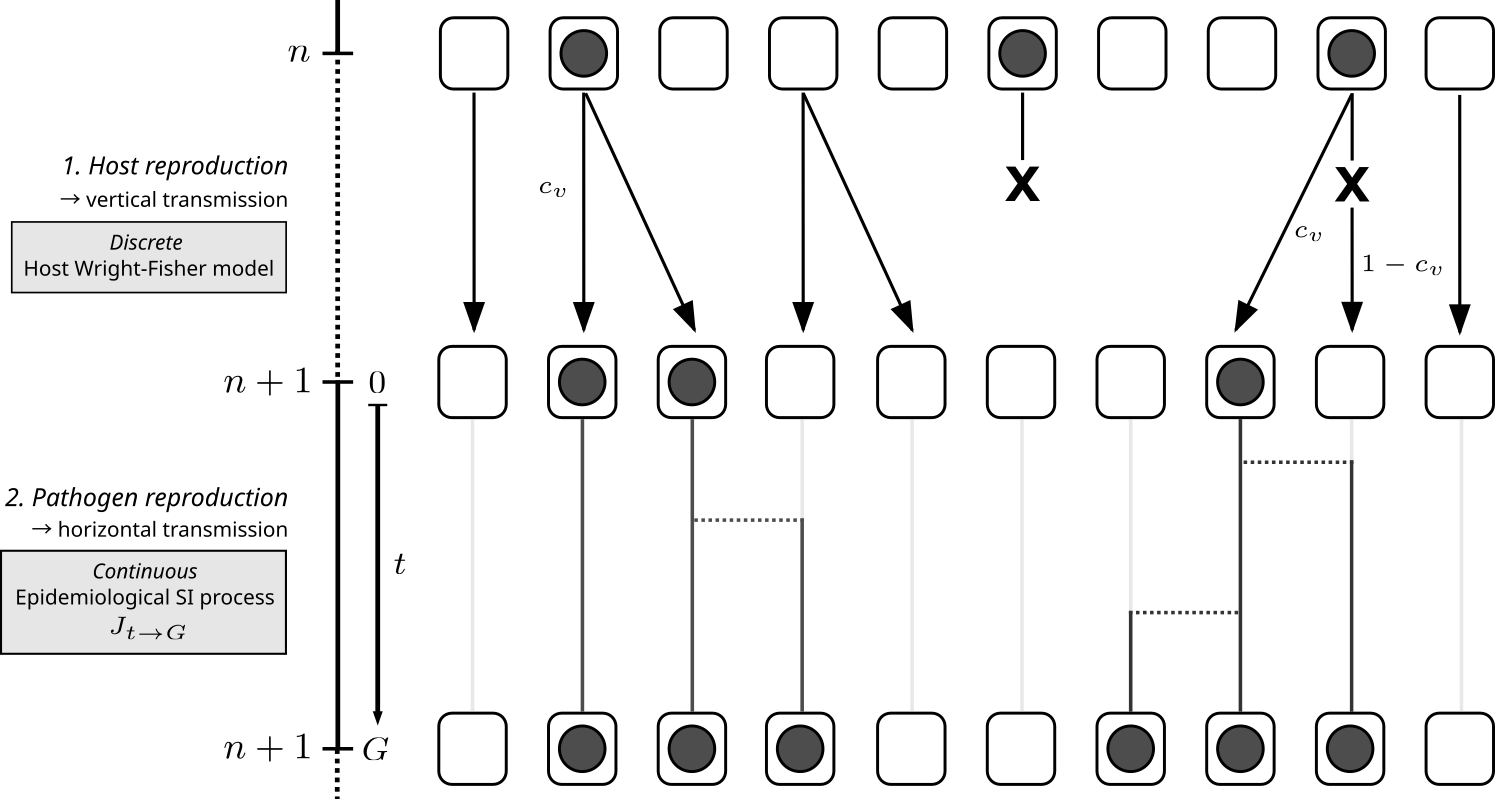
\includegraphics[width=1\linewidth]{../figures/nestedHostPathogen_WF_SI.png}
    \caption{Semi-discrete host-pathogen model with horizontal and vertical transmission. Pathogen can transmit vertically with probability $c_v$, following the host genealogy. Within each host generation there is a continuous epidemiological process $J_t$, modelling horizontal transmission through an SI infection model, determined by the contact rate $\beta$ and the duration of the epidemic $G$.}
    \end{figure}

    \textbf{Deterministic limit}\\
    Assuming the number of infected at the end of the generation \(n+1\) to be
    \begin{equation}
    X_{n+1} = I_{n+1} + K_{n+1}
    \end{equation}
    where \(I_{n+1}\) is the number of infected host offspring and \(K_{n+1}\) individuals are newly infected due to the epidemiological process \(\mathcal{J}_G\) in generation \(n+1\).
    If we take \(N\) to infinity, we get the deterministic limit of the model, and with \(x_n = X_n/N\) we have \(I_{n+1}/N \approx c_v x_n\). See notes for further details. For the stationary solution \(x_n = x_{n+1} = x\) we get
    \begin{equation}
    x = x^* = \frac{c_v - e^{-\beta G}}{c_v(1-e^{-\beta G})} 
    \end{equation}
    The value of \(x^*\) for values of \(c_v\), \(\beta\) and \(G\) are shown below. Values of \(x^* < 0\) are set to 0, as biologically, we require a positive fraction \(x\).
    \begin{figure}[H]
    \centering
    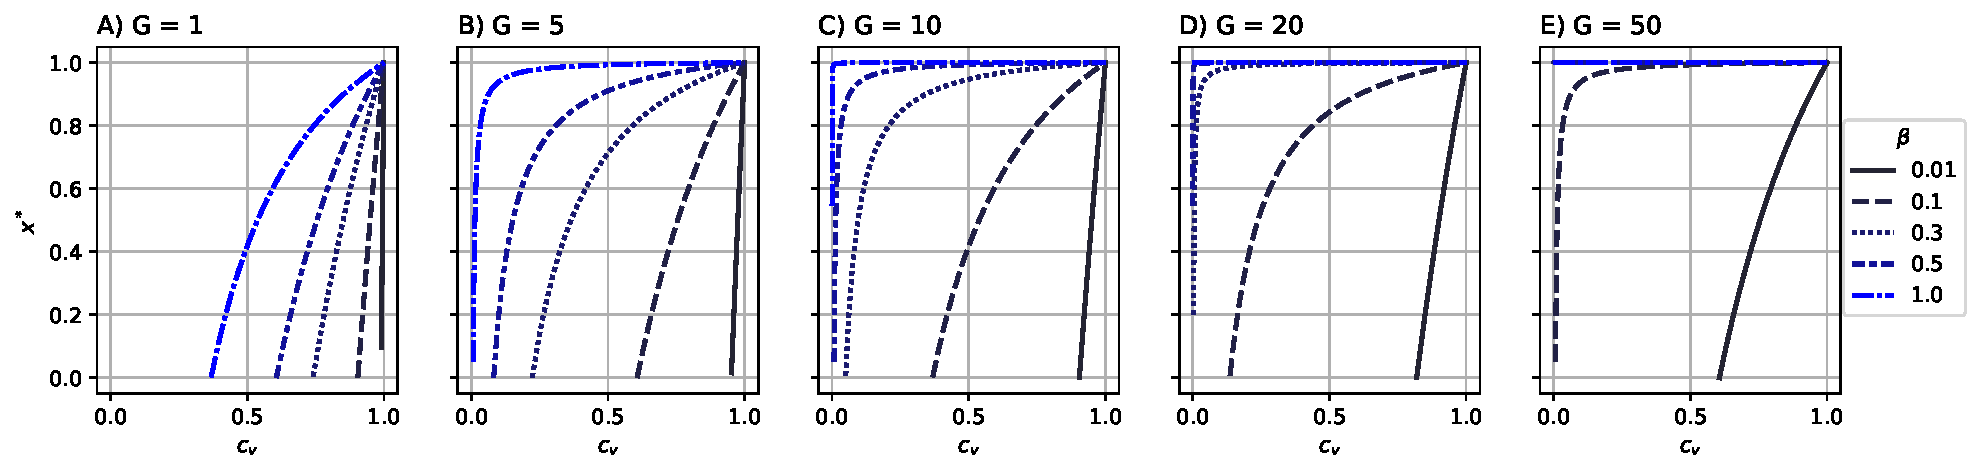
\includegraphics[width=\linewidth]{../maths/figures/x_equilibrium_vs_cv_perBeta_G.pdf}
    \caption{Behaviour of the equilibrium \(x^*\) for rates of vertical transmission \(c_v\) and horizontal contact rate \(\beta\) and epidemic time \(G\) (A-E).}
    \end{figure}
    \end{nofillbox}
    \begin{nofillbox}{Stochastic, individual-based simulations with \textit{SLiM 5}}
      This is the second column box. It sits perfectly parallel to the left one
    \end{nofillbox}
\end{tcbraster}



\section*{Discussion}

Lorem ipsum dolor sit amet, consectetur adipiscing elit. Interpret
the findings, discuss limitations, and connect the results to
previous work \parencite{example2020}.

\section*{Conclusion}

Lorem ipsum dolor sit amet, consectetur adipiscing elit. State the
main takeaway and the next step.

% ------------------------------------------------------------
% Footer: affiliations, funding, references, and logo
% ------------------------------------------------------------

\vfill

\begin{footerbox}
    \begin{minipage}{0.29\textwidth}
    \textbf{\fontsize{26}{32}\selectfont Funding}\\
    \vspace{0.4cm}
    {\fontsize{18}{23}\selectfont
    This work was supported by [funding agency / grant].}
    \end{minipage}
    % \hfill
    \begin{minipage}{0.50\textwidth}
    \textbf{\fontsize{26}{32}\selectfont Selected references}\\
    \vspace{0.4cm}
    {\fontsize{18}{23}\selectfont
    1. Author et al. (2023). Article title. \textit{Journal}.
    2. Author et al. (2024). Article title. \textit{Journal}.
  3. Author et al. (2025). Article title. \textit{Journal}.}
  
    \end{minipage}
\hfill
    \begin{minipage}{0.09\textwidth}
    \vfill
    \centering
    
\includegraphics[width=\linewidth]{./Universitaet_Logo_RGB.pdf}
    \end{minipage}
\end{footerbox}

\end{document}
